%%%%%%%%%%%%%%%%%%%%%%%%%%%%%%%%%%%%%%%%%%%%%%%%%%%%%%%%%%%%%%%%%%%%%%%%%%%%%%%

\chapter{INTRODUÇÃO}\label{ch:intro}

O Centro de Controle de Satélites (CCS) é um departamento pertencente ao Instituto Nacional de Pesquisas Espaciais (INPE) atualmente monitora e controla os seguintes satélites: a família do Satélite de Coleta de Dados (SCD), composta de dois satélites SCD-1 e SCD-2, e a família do Satélite Sino-Brasileiro de Recursos Terrestres (CBERS), com apenas o quinto satélite em operação atualmente, o CBERS-4.
Estes satélites realizam passagens sobre as estações terrenas do INPE, durante o qual o CCS recebe dados do estado do satélite, chamados de telemetrias, e envia telecomando, utilizados para controlar o satélite, bem como realiza atividades de manutenção e estimativa, como medidas de velocidade e posição de cada satélite~\cite{AzevedoAmbr:2010:ArSaTe}.

Dados de telemetria geralmente carregam medidas de sensores e verificações de saúde dos instrumentos, como temperatura das baterias, corrente de algum subsistema, se um dado equipamento está ativo ou não, bem como dados que os operadores e engenheiros acham necessários para a operação, entre outros~\cite{larsonSpaceMissionAnalysis1999}.
Estes dados precisam ser guardados por toda a vida do satélite, sendo que para satélites que estão em funcionamento por vários anos adquirem um volume de dados considerável, que não pode ser descartado.
No caso dos satélites da família SCD, o SCD-1 já estando operacional por mais de 25 anos, e continuando a gerar dados, com um volume aproximado de 7GB por ano.

Para satélites mais complexos como os da família CBERS, que possuem mais de 4 mil telemetrias sendo monitoradas, geram um volume de dados cuja análise não é trivial, e só pode ser feita por especialistas no funcionamento do satélite.
Com os lançamentos futuros do CBERS-4A e do Amazônia-1, o volume de dados e a complexidade da análise dos mesmos deve aumentar, criando novas necessidades de operação~\cite{JulioFoAmbrFerrLour:2017:ChImSp}.

{\color{cerulean}

A figura~\ref{fig:datagenest} mostra uma uma estimativa simples da geração histórica de dados de telemetria no CCS.
Essa estimativa foi feita utilizando dos dados não compressos a partir da disponibilidade dos mesmos.
Ela também assume que o Amazônia-1 vai gerar um volume de dados de telemetria similar ao gerado do CBERS.

\begin{figure}[!htb]
	\caption{Estimativa de geração anual de dados pelos satélites do INPE}\label{fig:datagenest}
	\vspace{4mm}
	\begin{center}
		\resizebox{14cm}{!}{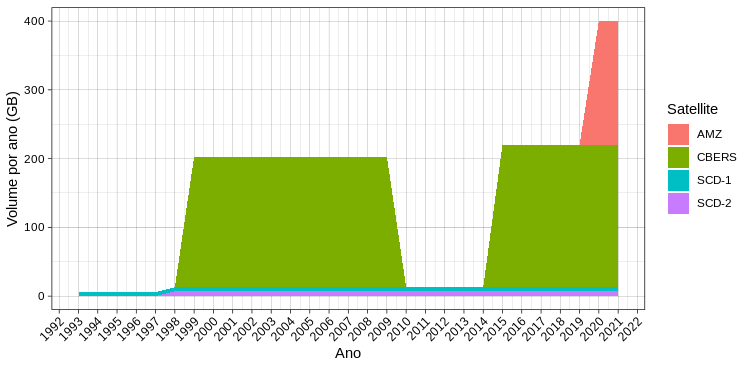
\includegraphics{Figuras/DataGenSatYear.png}}
	\end{center}
	\vspace{2mm}
	\legenda{Volume estimado de geração de dados por cada ano de operação de cada satélite.}
	\FONTE{Produção do autor.}
\end{figure}

Dessa estimativa, podemos obter o total de dados de telemetria disponíveis para a análise no CCS considerando uma taxa constante dos satélites, apresentados na figura~\ref{fig:totaldatagen}.
É importante ressaltar que a grande maioria desses dados não está disponível para consulta pelo usuário, visto que somente os dados de alguns poucos anos da operação estão disponíveis para os operadores e engenheiros, necessitando de trabalho significativo para analisar dados do passado.

\begin{figure}[!hb]
	\caption{Estimativa do volume de dados histórico de telemetria de todos os satélites}\label{fig:totaldatagen}
	\vspace{4mm}
	\begin{center}
		\resizebox{13cm}{!}{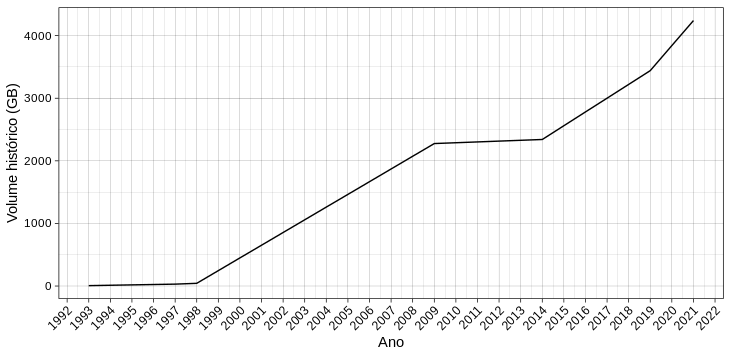
\includegraphics{Figuras/VolumeToYear.png}}
	\end{center}
	\vspace{2mm}
	\legenda{Volume total estimado de dados de telemetria gerados por todos os satélites.}
	\FONTE{Produção do autor.}
\end{figure}

Esses dados devem ser propriamente tratados para que não virem ``\textit{dark data}'', termo que denota quaisquer tipo de dados que não são de fácil acesso para os seus usuários em potencial~\cite{heidornSheddingLightDark2008}.

Esses dados entram na definição de \textit{Big Data}, pois possuem um grande volume, são gerados continuamente, possuem formatos diversos, sua análise é de alto valor e existe uma incerteza quanto a qualidade dos dados devido a problemas de comunicação e degradação dos instrumentos.
Essas características são denotadas pelos cinco Vs do \textit{Big Data}: Volume, Variedade, Velocidade, Valor e Veracidade~\cite{kacfahemaniUnderstandableBigData2015}.

Considerando que todos os dados já estivessem no banco de dados, propriamente formatados e prontos para a análise, ainda teríamos grandes problemas: com um banco de dados na ordem dos \textit{terabytes}, consultas multidimensionais ou que precisem de dados de vários anos poderiam demorar dias, ou mais, para serem executadas.

}

Deste modo, é necessário criar uma estrutura que permita a análise e consulta desses dados de uma forma estruturada e que tenha desempenho satisfatório.
As tecnologias de \textit{Data Warehouse} (DW) e \textit{Online Analytical Processing} (OLAP) tem demonstrado capacidade e experiência para atingir esses objetivos~\cite{bimonteOpenIssuesBig2016}, inclusive na área espacial~\cite{yvernesCopernicusGroundSegment2018}.
Essas tecnologias executam a generalização de dados agregando enormes quantidade de dados em vários níveis de abstração, assim tornam elementos essenciais de apoio à decisão e atraem a atenção tanto da indústria como das comunidades de pesquisa.
Sistemas OLAP, que são tipicamente dominados por consultas complexas que envolvem operadores \textit{group-by} e operadores de agregações, são as principais características entre essas ferramentas.

Sistemas OLAP são baseados em um modelo multidimensional chamado de cubo de dados, que é uma generalização do operador \textit{group-by} sobre todas as combinações possíveis das dimensões, com variados níveis de granularidade~\cite{grayDataCubeRelational1996}.
Cada combinação é chamada de um subcubo, que correspondem a um conjunto de células descritas como tuplas sobre as dimensões do subcubo.
Além das dimensões, cada tupla contém um fato, também chamado de medida, que representa o que será medido no processo de análise.

Cada dimensão pode estar organizada em uma hierarquia para facilitar a análise.
Por exemplo, uma dimensão tempo pode ser dividida em ``dia < mês < ano'', com ano sendo o nível mais genérico.
Essa prática visa facilitar a interpretação dos dados pelos usuários.
Medidas são atributos atributos associados a uma combinação de dimensões, sendo geradas de forma estatística.

Tecnologias OLAP são caracterizadas pela habilidade em responder consultas de apoio a decisão de forma eficiente.
Para atingir isso, o cubo de dados deve ser materializado antes da execução da consulta.
Isso significa que as combinações de dimensões são computadas previamente, assim gerando o cubo de dados completo.
Porém, essa abordagem possui um custo computacional exponencial em relação ao número de dimensões, assim a materialização completa do cubo envolve um grande número de células e um tempo substancial para a sua execução.

Dados de satélite são caracterizados pela sua alta dimensionalidade, onde um satélite pode precisar rastrear milhares de telemetrias.
Por exemplo, supondo um satélite com $n = 100$ telemetrias, e cada telemetria representando uma dimensão, teremos $2^{100}$ possíveis subcubos para a implementação de um cubo de dados.
Supondo uma cardinalidade, o número de valores diferentes em cada telemetria, como sendo de $100$, teremos $101^{100} \approx 10^{200}$ células para cada dimensão.
{\color{cerulean}
Devido ao controle ativo pelos operadores de satélite, os dados são concentrados em alguns valores que se repetem frequentemente, sendo que isso é chamado de \textit{skew}.
}

Dessa forma, conseguir calcular e manter um cubo de dados é um problema exponencial, e reduzir o seu consumo de memória e tempo de computação é de fundamental importância para desenvolver um sistema OLAP.
Para a área espacial essa necessidade é maior: a maior parte dos algoritmos de computação do cubo tem problemas em lidar com mais do que 15 dimensões~\cite{silva:2015:abordagensParaCubo}.

\section{Objetivos}\label{ch:intro:obj}

{\color{cerulean}

Assim, este trabalho tem como objetivo estabelecer um método para processamento de cubos de dados para a área espacial, para que o processamento de consultas OLAP sejam executadas de forma eficiente considerando-se a alta dimensionalidade, elevado número de tuplas, alto \textit{skew} e alta cardinalidade dos dados.

Assim é necessário identificar quais são as consultas de interesse dos operadores de satélite e quais são as análises que devem ser feitas pelos mesmos.
Disso será criada uma representação dimensional dos dados de telemetria em uma estrutura do cubo de dados, e  algoritmos de construção do cubo devem ser avaliados para identificar qual é o mais apropriado para responder as consultas.

Como resultados esperados deste trabalho teremos a avaliação dos algoritmos de construção do cubo nos dados altamente dimensionais, teremos as consultas identificadas e a adequabilidade do uso de cubo de dados como uma solução para operadores de satélites.

}

\section{Organização da proposta}\label{ch:intro:org}

Os capítulos restantes desta proposta estão organizados da seguinte maneira:

\begin{itemize}
	\item{Capítulo 2}: Este capítulo apresenta os conceitos e fundamentos teóricos desta proposta, como os conceitos relevantes de operação de satélites, \textit{Data Warehouse}, \textit{Big Data} e do Cubo de Dados.
	\item{Capítulo 3}: Neste capítulo os trabalhos correlatos de Cubo de Dados são apresentados, bem como as arquiteturas que outros operadores de satélite estão implementando.
	\item{Capítulo 4}: Neste capítulo a proposta é apresentada e seus conceitos principais explicados.
	\item{Capítulo 5}: Esse capítulo apresenta os resultados alcançados até o momento.
	\item{Capítulo 6}: Com base nos resultados intermediários alcançados, esse capítulo apresentará as conclusões obtidas, bem como as direções de implementação para o resto do trabalho.
\end{itemize}

